% -*- latex -*-
%%%%%%%%%%%%%%%%%%%%%%%%%%%%%%%%%%%%%%%%%%%%%%%%%%%%%%%%%%%%%%%%
%%%%
%%%% This TeX file is part of the course
%%%% Introduction to Scientific Programming in C++/Fortran2003
%%%% copyright 2017-2023 Victor Eijkhout eijkhout@tacc.utexas.edu
%%%%
%%%% function.tex : functions
%%%%
%%%%%%%%%%%%%%%%%%%%%%%%%%%%%%%%%%%%%%%%%%%%%%%%%%%%%%%%%%%%%%%%

A~\indexterm{function}
(or~\emph{subprogram}\index{subprogram|see{function}}) is a way to
abbreviate a block of code and replace it by a single line.
This is foremost a code structuring device: by giving a function a
relevant name you introduce the terminology of your application into
your program.

\begin{itemize}
\item Find a block of code that has a clearly identifiable function.
\item Turn this into a function: the function definition will contain
  that block, with a header that names it.
\item The function is called by its name.
\end{itemize}

\begin{block}{Introducing a function}
  \vskip0pt
  \label{sl:func-scheme}
  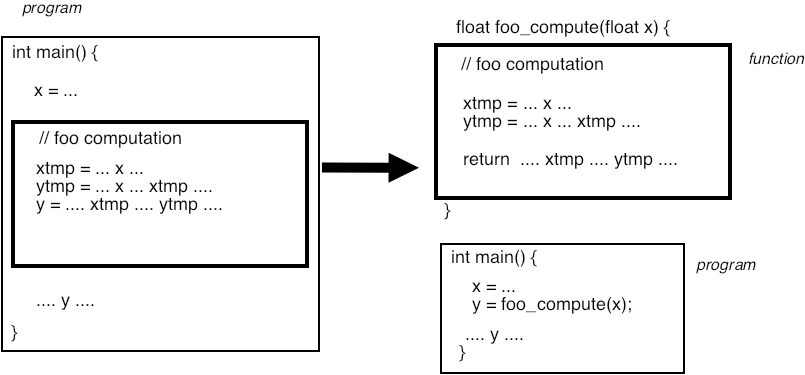
\includegraphics[scale=.4]{functiondiagram}
\end{block}

\begin{slide}{Why functions?}
  \label{sl:function-intro}
  Functions are an abstraction mechanism.
  \begin{itemize}
  \item Code fragment with clear function:
  \item Turn into \emph{subprogram}: function \emph{definition}.
  \item Use by single line: function \emph{call}.
  \item Abstraction: you have introduced a \textbf{name} for a
    section of code.
  \end{itemize}
\end{slide}

By introducing a function name you have introduced
\indexterm{abstraction}: your program now uses terms related to your
problem, and not
just the basic control structures such as \lstinline{for}.
With objects (chapter~\ref{ch:object}) you will learn further abstractions,
so that instead of integers and arrays
your program will use application terms,
such as \lstinline{Point} or \lstinline{Line}.

\Level 0 {Function definition and call}

There are two aspects to a function:
\begin{itemize}
\item
  The \indextermbus{function}{definition} is done once, typically
  above the main program;
\item a \indextermbus{function}{call} to any function can happen
  multiple times, inside the main program or inside other functions.
\end{itemize}

Let's consider a simple example program,
in which we introduce functions.
We code the \indexterm{bisection} algorithm for finding
the root of a function;
see section~\ref{sec:root-bisection} for details.

\begin{block}{Program without functions}
  \label{sl:nodef-nocall}
  Example: zero-finding through bisection.
  \[ \mathop{?}_x\colon f(x)=0,\qquad f(x)=x^3-x^2-1 \]
  (where the question mark quantor stands for `for which~$x$').

  First attempt at coding this: everything in the main program.
  \snippetwithoutput{bisect1main}{func}{bisect1}
\end{block}

We modularize this in two steps.
The first function we introduce is the objective function~$f(x)$.

\begin{block}{Introducing functions, step 1}
  \label{sl:def-call1}
  \begin{multicols}{2}
Introduce a function for the expression \n{m*m*m - m*m-1}:
\verbatimsnippet{bisect2func}
Used in main:
\columnbreak
\verbatimsnippet{bisect2main}
  \end{multicols}
\end{block}

Next we introduce a function for the zero-finding algorithm.

\begin{block}{Introducing functions, step 2}
  \label{sl:def-call2}
  \begin{multicols}{2}
    Function:
    \verbatimsnippet{bisect3func}
    \columnbreak
    New main:
    \verbatimsnippet{bisect3main}
    \vfill
  \end{multicols}
\end{block}

The main now no longer contains any implementation details,
such as local variables, or method used.
This makes the main program shorter and more elegant:
we have moved the variables for the midpoint inside the function.
These are implementation details and should not be in the main program.

In this example, the function definition consists of:
\begin{itemize}
\item The  keyword \lstinline{float} indicates that the function 
  returns a \lstinline{float} result to the calling code.
\item The name \lstinline{find_zero_between} is picked by you.
\item The parenthetical part \lstinline{(float l,float r)} is called the `parameter list':
  it says that the function takes two floats as input.
  For purposes of the function,
  the floats will have the names~\lstinline{l,r},
  regardless any names in the main program.
\item The `body' of the function, the code that is going to be
  executed, is enclosed in curly brackets.
\item A `return' statement that transfers a computed result out of the function.
\end{itemize}

\Level 1 {Formal definition of a function definition}

Formally, a~function definition
consists of:

\begin{itemize}
\item \indextermbusdef{function}{result type}: you need to indicate
  the type of the result;
\item name: you get to make this up;
\item zero or more \indextermbus{function}{parameters}. These describe
  how many \indextermbus{function}{arguments} you need to supply as
  input to the function. Parameters consist of a type and a name. This
  makes them look like variable declarations, and that is how they
  function. Parameters are separated by commas.

  Then follows the:
\item \indextermbusdef{function}{body}: the statements that make up
  the function. The function body is a \emph{scope}: it can have local
  variables. (You can not nest function definitions.)
\item a \indextermdef{return} statement. Which doesn't have to be
  the last statement, by the way.
\end{itemize}

\begin{slide}{Anatomy of a function definition}
  \label{sl:func-anatomy}

\begin{lstlisting}
void write_to_file(int i,double x) { /* ... */ }
float euler_phi(int i,bool tf) { /* ... */ return x; }
\end{lstlisting}

  \begin{itemize}
  \item Result type: what's computed.\\ \lstinline{void} if no result
  \item Name: make it descriptive.
  \item Parameters: zero or more.\\
    \lstinline{int i,double x,double y}\\
    These act like variable declarations.
  \item Body: any length. This is a scope.
  \item Return statement: usually at the end, but can be anywhere; the
    computed result. Not necessary for a \lstinline{void} function.
  \end{itemize}
\end{slide}

The function can then be used in the main program, or in another function.

A function body defines a
\emph{scope}\index{scope!of function body}%
\index{function!defines scope}:
the local variables of the function calculation are invisible to the
calling program.

Functions can not be nested: you can not define a function inside the
body of another function.

\Level 1 {Function call}

The \indextermbus{function}{call} consists of
\begin{itemize}
\item The name of the function, and
\item In between parentheses, any input argument(s).
\end{itemize}
The function call can stand on its own, or can be on the right-hand-side
of an assignment.

\begin{exercise}
  \label{ex:bisect-extend}
  Make the bisection algorithm more elegant
  by introducing functions \lstinline+new_l+, \lstinline+new_r+ used as:
\begin{lstlisting}
l = new_l(l,mid,fmid);
r = new_r(r,mid,fmid);
\end{lstlisting}
\skeleton{bisect}

Question: you could leave out \lstinline+fmid+ from the functions.
Write this variant. Why is this not a good idea?
\end{exercise}

\begin{block}{Function call}
  \label{sl:func-call}
  The function call
  \begin{enumerate}
  \item copies the value of the \indextermbus{function}{argument}
    to the \indextermbus{function}{parameter};
  \item causes the function body to be executed, and
  \item the function call is replaced by whatever you \lstinline{return}.
  \item (If the function does not return anything, for instance because
    it only prints output, you declare the return type to be \indexc{void}.)
  \end{enumerate}
\end{block}

To introduce two formal concepts:
\begin{itemize}
\item A function definition can have zero or more \indextermdef{parameter}s,
  or \indextermsub{formal}{parameter}s.
  These function as variable definitions local to the function.
\item The function call has a corresponding number of \indextermdef{argument}s,
  or \indextermsub{actual}{parameter}s.
\end{itemize}

\Level 1 {Why use functions?}

In many cases, code that is written using functions can also be
written without. So why would you use functions? There are several
reasons for this.

Functions can be motivated as making your code more structured and intelligible.
The source where you use the function call becomes shorter,
and the function
name makes the code more descriptive. This is sometimes called
`self-documenting code'.

Sometimes introducing a function can be motivated from a point of
\indexterm{code reuse}: if the same block of code appears in two
places in your source (this is known as
\indextermbus{code}{duplication}), you replace this by one function
definition, and two (single line) function calls.

\begin{block}{Code reuse}
  \label{sl:reuse}
Suppose you do the same computation twice:
\begin{lstlisting}
double x,y, v,w;
y = ...... computation from x .....
w = ...... same computation, but from v .....
\end{lstlisting}
With a function this can be replaced by:
\begin{lstlisting}
double computation(double in) {
  return .... computation from `in' ....
}

y = computation(x);
w = computation(v);
\end{lstlisting}
\end{block}

\begin{block}{Code reuse}
  \label{sl:function-reuse}
Example: multiple norm calculations:
  \begin{multicols}{2}
    \small
    Repeated code:
\begin{lstlisting}
float s = 0;
for (int i=0; i<x.size(); i++)
  s += abs(x[i]);
cout << "One norm x: " << s << endl;
s = 0;
for (int i=0; i<y.size(); i++)
  s += abs(y[i]);
cout << "One norm y: " << s << endl;
\end{lstlisting}
\vfill\columnbreak
becomes:
\begin{lstlisting}
float OneNorm( vector<float> a ) {
  float sum = 0;
  for (int i=0; i<a.size(); i++)
    sum += abs(a[i]);
  return sum;
}
int main() {
  ... // stuff
  cout << "One norm x: "
       << OneNorm(x) << endl;
  cout << "One norm y: " 
       << OneNorm(y) << endl;
\end{lstlisting}
  \end{multicols}
  (Don't worry about array stuff in this example)
\end{block}

A final argument for using functions is code maintainability:
\begin{itemize}
\item Easier to debug: if you use the same (or roughly the same) block
  of code twice, and you find an error, you need to fix it twice.
\item Maintainance: if a block occurs twice, and  you change something in such a block
  once, you have to remember to change the other occurrence(s) too.
\item Localization: any variables that only serve the calculation in
  the function now have a limited \indexterm{scope}.
\begin{lstlisting}
void print_mod(int n,int d) {
  int m = n%d;
  cout << "The modulus of " << n << " and " << d 
       << " is " << m << endl;
\end{lstlisting}
\end{itemize}

\begin{slide}{Why functions?}
  \label{sl:func-why}
  \begin{itemize}
  \item Easier to read: use application terminology
  \item Shorter code: reuse
  \item Cleaner code: local variables are no longer in the main program.
  \item Maintainance and debugging
  \end{itemize}
\end{slide}

\begin{review}
  \label{rev:func-why}
  True or false?
  \begin{itemize}
  \item The purpose of functions is to make your code shorter.
    \slackpollTF+Functions are to make your code shorter+
  \item Using functions makes your code easier to read and understand.
    \slackpollTF+Functions make your code easier to understand+
  \item Functions have to be defined before you can use them.
    \slackpollTF+Functions have to be defined before use+
  \item Function definitions can go inside or outside the main program.
    \slackpollTF+Function definitions can go in or out main+
  \end{itemize}
\end{review}

\Level 0 {Anatomy of a function definition and call}

Loosely, a function takes input and computes some result which is then returned.
Just some simple examples:

\begin{multicols}{2}
\begin{lstlisting}
int compute( float x, char c ) {
    /* code */
    return somevalue;
};
// in main:
i = compute(x,'c');
\end{lstlisting}
\columnbreak
\begin{lstlisting}
void compute( float x, char c ) {
    /* code */
};
// in main:
compute(x,'c');
\end{lstlisting}
\end{multicols}

So we need to discuss the function definition and its use.


\Level 0 {Definition vs declaration}

The C++ \emph{compiler} translates your code in
\emph{one pass}\index{compiler!one pass}: it goes from top to
bottom through your code. This means you can not make reference to
anything, such as a function name, that you haven't defined yet.
For this reason, in the examples so far we put the function definition
before the main program.

There is another solution.
For the compiler to judge whether a function call is legal
it does not need the full function definition:
it can proceed once it know the name of the function, and the types of
the inputs and result.
This information is sometimes called a
\indextermbus{function}{header},
\indextermbus{function}{prototype},
or \indextermbus{function}{signature},
but the technical term is a \indextermsub{function}{declaration}.

In the following example we put the function declaration before the main program,
and the full function definition after it:

\begin{block}{Declaration first, definition last}
  \label{sl:proto-first}
  Some people like the following style of defining a function:
\begin{lstlisting}
// declaration before main
int my_computation(int);

int main() {
  int result;
  result = my_computation(5);
  return 0;
};

// definition after main
int my_computation(int i) {
   return i+3;
}
\end{lstlisting}
This is purely a matter of style.
\end{block}

See chapter~\ref{ch:proto} for more details.

\Level 0 {Void functions}

Some functions do not return a result value,
for instance because only write
output to screen or file. In that case you define the function to be
of type \indexcdef{void}.

\begin{block}{Functions without input, without return result}
  \label{sl:func-ex1}
\begin{lstlisting}
void print_header() {
  cout << "****************" << endl;
  cout << "* Output       *" << endl;
  cout << "****************" << endl;
  }
int main() {
  print_header();
  cout << "The results for day 25:" << endl;
  // code that prints results ....
  return 0;
}
\end{lstlisting}
\end{block}

\begin{block}{Void function with input}
  \label{sl:func-ex2}
\begin{lstlisting}
void print_result(int day,float value) {
  cout << "****************" << endl;
  cout << "* Output       *" << endl;
  cout << "****************" << endl;
  cout << "The results for day " << day << ":" << endl;
  cout << "    " << value << endl;
  }
int main() {
  print_result(25,3.456);
  return 0;
}
\end{lstlisting}
\end{block}

\begin{review}
  \label{rev:func-param}
  True or false?
  \begin{itemize}
  \item A function can have only one input
    \slackpollTF+Function can have only one input+
  \item A function can have only one return result
    \slackpollTF+Function can have only one return result+
  \item A void function can not have a \lstinline{return} statement.
    \slackpollTF+Void function can not have 'return'+
  \end{itemize}
\end{review}

%%%%
%%%% Parameter passing
%%%%
\Level 0 {Parameter passing}
\label{sec:passing}
\index{parameter|seealso{function, parameter}}
%\input parampassing

C++~functions resemble mathematical functions: you have seen that a
function can have an input and an output. In fact, they can have
multiple inputs, separated by commas, but they have only one
output.
\[ a = f(x,y,i,j) \]

We start by studying functions that look like these mathematical
functions. They involve a \indextermbus{parameter}{passing} mechanism
called
\emph{passing by value}\index{parameter!passing by value}.
%
Later we will then look at
\emph{passing by reference}\index{parameter!passing by reference}.

\Level 1 {Pass by value}
\label{sec:pass-value}
\index{pass by value|see{parameter, passing by value}}

The following style of programming is very much inspired by
mathematical functions, and is known as \indextermdef{functional
  programming}\footnote {There is more to functional programming. For
  instance, strictly speaking your whole program needs to be based on
  function calling; there is no other code than function definitions
  and calls.}.
\begin{itemize}
\item A function has one result, which is returned through a return
  statement. The function call then looks like
\begin{lstlisting}
y = f(x1,x2,x3);
\end{lstlisting}
\item Example:
  \snippetwithoutput{passvalue}{func}{passvalue}
\item The definition of the C++ parameter passing mechanism says that
  input arguments are copied to the function, meaning that they don't
  change in the calling program:
  %
  \snippetwithoutput{passvaluelocal}{func}{passvaluelocal}

\end{itemize}

We say that the input argument is
\emph{passed by value}\index{parameter!pass by value|textbf}:
its value is copied into the
function.  In this example, the function parameter \lstinline{x} acts as a
local variable in the function, and it is initialized with a copy of
the value of \lstinline{number} in the main program.

\begin{exercise}
  \label{ex:swapbyvalue}
  Write two functions
\begin{lstlisting}
int biggest(int i,int j);
int smallest(int i,int j);
\end{lstlisting}
  and a program that prints the results:
\begin{lstlisting}
int i = 5, j = 17;
cout ... biggest(i,j) ...
cout ... smallest(i,j) ...
\end{lstlisting}
\end{exercise}

\begin{slide}{Mathematical type function}
  \label{sl:func-functional}
  Pretty good design:
  \begin{itemize}
  \item pass data into a function,
  \item return result through \lstinline{return} statement.
  \item Parameters are copied into the function. (Cost of copying?)
  \item \indexterm{pass by value}
  \item `functional programming'
  \end{itemize}
\end{slide}

\begin{slide}{Pass by value example}
  \label{sl:func-functional-ex}
  Note that the function alters its parameter \lstinline{x}:
  %
  \snippetwithoutput{passvalue}{func}{passvalue}
  %
  but the argument in the main program is not affected.
\end{slide}

Passing a variable to a routine passes the value; in the routine, the
variable is local. So, in this example
the value of the argument is not changed:

\snippetwithoutput{localparm}{func}{localparm}

\begin{exercise}
  If you are doing the prime numbers project (chapter~\ref{ch:prime}) you can
  now do exercise~\ref{ex:prime:func}.
\end{exercise}

\begin{exercise}
  If you are doing the zero-finding project (chapter~\ref{ch:zerofind})
  you can now do exercise~\ref{ex:newton-root}.
\end{exercise}

\Level 1 {Pass by reference}
\label{sec:pass-by-ref}
\index{pass by reference|see{parameter, passing by reference}}
  
Having only one output is a limitation on functions. Therefore there
is a mechanism for altering the input parameters and returning
(possibly multiple) results that way. You do this by not copying
values into the function parameters, but by turning the function
parameters into aliases of the variables at the place where the
function is called.

We need the concept of a \indextermdef{reference}:
another variable to refers to the same `thing' as another,
already existing, variable.

\begin{plainblock}{Reference}
  \label{sl:cpp-reference}
  A reference is indicated with an ampersand in its definition, and it
  acts as an alias of the thing it references.
  %
  \snippetwithoutput{refint}{basic}{ref}
  %
  (You will not use references often this way.)
\end{plainblock}

\begin{block}{Create reference by initialize}
  \label{sl:cpp-ref-define}
  Correct:
\begin{lstlisting}
float x{1.5};
float &xref = x;
\end{lstlisting}
Not correct:
\begin{lstlisting}
float x{1.5};
float &xref; // WRONG: needs to initialized immediately
xref = x;

float &threeref = 3; // WRONG: only reference to `lvalue'
\end{lstlisting}
\end{block}

\begin{comment}
  \begin{advanced}
    If you already know about pointers, you may wonder about the similarities.
    \begin{itemize}
    \item There are no `null' references. There is a \indexc{nullptr}.
    \item References are bound when they are created.
    \item You can not change what a reference is bound to;
      the pointer target can change.
    \item Reference syntax is cleaner.
    \item Pointer use has implications about ownership: use only for specific purposes.
    \end{itemize}
  \end{advanced}
\end{comment}

\begin{slide}{Reference vs pointer}
  \label{sl:ref-vs-ptr}
  \begin{itemize}
  \item There are no `null' references.\\
    (There is a \indexc{nullptr}, but that has nothing to do with references.)
  \item References are bound when they are created.
  \item You can not change what a reference is bound to;\slidebreak
    a~pointer target can change.
  \end{itemize}
\end{slide}

You can make a function parameter into a reference of a variable in
the main program. This makes the function parameter into another name referring
to the same thing.

\begin{block}{Parameter passing by reference}
  \label{sl:pass-by-ref}
The function parameter \lstinline{n} becomes a reference to the variable \lstinline{i}
in the main program:
\lstset{numbers=left,numberstyle=\tiny}
\begin{lstlisting}
void f(int &n) {
  n = /* some expression */ ;
};
int main() {
  int i;
  f(i);
  // i now has the value that was set in the function
}
\end{lstlisting}
 Reference syntax is cleaner than C `pass by reference'
\end{block}

Using the ampersand, the parameter is
\emph{passed by reference}\index{parameter!passing by reference|textbf}:
instead of copying the value, the function receives a reference,
so that the parameter becomes a reference to the thing
in the \indexterm{calling environment}.

\begin{remark}
  The \emph{pass by reference mechanism in C}%
  \index{parameter!passing by reference! in C}
  was different and should not be used in~C++. In fact it was not a
  true pass by reference, but passing an address by value.
  If you do need the address of a variable, use \indexc{addressof}
  from the \indexheader{memory} header, since the ampersand operator
  can be overloaded.
\end{remark}

\begin{remark}
  We sometimes use the following terminology for function parameters:
  \begin{itemize}
  \item \emph{input}\index{parameter!input|textbf} parameters: passed by
    value, so that it only functions as input to the function, and no
    result is output through this parameter;
  \item \emph{output}\index{parameter!output|textbf} parameters: passed
    by reference so that they return an `output' value to the program.
  \item \emph{throughput}\index{parameter!throughput|textbf} parameters:
    these are passed by reference, and they have an initial value when
    the function is called. In C++, unlike Fortran, there is no real
    separate syntax for these.
  \end{itemize}
\end{remark}

\begin{block}{Pass by reference example 1}
  \label{sl:pass-reference1}
  \snippetwithoutput{setbyref}{basic}{setbyref}
  Compare the difference with leaving out the reference.
\end{block}

\begin{slide}{Results other than through return}
  \label{sl:func-err-return}
  Also good design:
  \begin{itemize}
  \item Return no function result,
  \item or return \indexterm{return status} (0~is success, nonzero various
    informative statuses), and
  \item return other information by changing the parameters.
  \item \emph{pass by reference}
  \item Parameters are sometimes classified `input', `output', `throughput'.
  \end{itemize}
\end{slide}

As an example, consider a function that tries to read a value from a
file. With anything file-related, you always have to worry about the
case of the file not existing and such. So our function returns:
\begin{itemize}
\item a boolean value to indicate whether the read succeeded, and
\item the actual value if the read succeeded.
\end{itemize}
The following is a common idiom, where the success value is returned
through the \lstinline{return} statement, and the value through a parameter.

\begin{block}{Pass by reference example 2}
  \label{sl:pass-reference2}
\footnotesize
\begin{lstlisting}
bool can_read_value( int &value ) {
  // this uses functions defined elsewhere
  int file_status = try_open_file();
  if (file_status==0) 
    value = read_value_from_file();
  return file_status==0;
}

int main() {
  int n;
  if (!can_read_value(n)) {
    // if you can't read the value, set a default
    n = 10;
  }
  ..... do something with 'n' ....
\end{lstlisting}
\end{block}

This latter example can also be solved,
perhaps more idiomatically, with \lstinline+std::optional+;
section~\ref{sec:std-optional}.

\begin{exercise}
  \label{ex:swap}
  Write a \lstinline{void} function \lstinline{swap} of two parameters that
  exchanges the input values:
  \snippetwithoutput{swapmain}{func}{swap}
\end{exercise}

\begin{exercise}
  \label{ex:div-remain}
  Write a divisibility function that takes a number and a divisor, and gives:
  \begin{itemize}
  \item a \lstinline{bool} return result indicating that the number is
    divisible, and
  \item a remainder as output parameter.
  \end{itemize}
  \snippetwithoutput{divistest}{func}{divisible}
\end{exercise}

\begin{exercise}
  \label{ex:geom-basic}
  If you are doing the geometry project, you should now do the exercises
  in section~\ref{sec:geom-basic}.
\end{exercise}

\Level 0 {Recursive functions}
\label{sec:recursion}
\index{recursion|see{function, recursive}}
\index{function!recursive|seealso{recursion}}

In mathematics, sequences are often recursively defined. For instance,
the sequence of factorials $n\mapsto f_n\equiv n!$ can be defined as
\[ f_0=1,\qquad \forall_{n>0}\colon f_n=n\times f_{n-1}. \]
Instead of using a subscript, we write an argument in parentheses
%
\[ F(n) = 
\begin{cases}
  n \times F(n-1) & \hbox{if $n>0$} \\
  1 &\hbox{otherwise} 
\end{cases}
\]
%
This is a form that can be translated into a C++ function.
The header of a factorial function can look like:
\begin{lstlisting}
int factorial(int n)
\end{lstlisting}
So what would the
function body be? We need a \lstinline{return} statement, and what we return
should be $n \times F(n-1)$:
\begin{lstlisting}
int factorial(int n) {
  return n*factorial(n-1);
} // almost correct, but not quite
\end{lstlisting}
So what happens if you write
\begin{lstlisting}
int f3; f3 = factorial(3);
\end{lstlisting}
Well,
\begin{itemize}
\item The expression \lstinline{factorial(3)} calls the \lstinline{factorial}
  function, substituting~\lstinline{3} for the argument~\lstinline{n}.
\item The return statement returns \lstinline{n*factorial(n-1)}, in this case
  \lstinline{3*factorial(2)}.
\item But what is \lstinline{factorial(2)}? Evaluating that expression means
  that the \lstinline{factorial} function is called again, but now with \lstinline{n}
  equal to~2.
\item Evaluating \lstinline{factorial(2)} returns \lstinline{2*factorial(1)},\ldots
\item \ldots~which returns \lstinline{1*factorial(0)},\ldots
\item \ldots~which returns~\ldots
\item Uh oh. We forgot to include the case where \lstinline{n} is zero. Let's
  fix that:
\begin{lstlisting}
int factorial(int n) {
  if (n==0)
    return 1;
  else
    return n*factorial(n-1);
}
\end{lstlisting}
\item Now \lstinline{factorial(0)} is~1, so \lstinline{factorial(1)} is
  \lstinline{1*factorial(0)}, which is~1,\ldots
\item \ldots~so \lstinline{factorial(2)} is~2, and \lstinline{factorial(3)} is~6.
\end{itemize}

\begin{slide}{Recursion}
  \label{sl:func-recur}
  A function is allowed to call itself, making it a \indextermsubdef{recursive}{function}.
  For example, factorial:
  \[ 5! = 5\cdot 4 \cdot \cdots \cdot 1 = 5 \times 4! \]
  You can define factorial as
  \[ F(n) = n \times F(n-1) \qquad \hbox{if $n>1$, otherwise~$1$} \]
\begin{lstlisting}
int factorial( int n ) {
  if (n==1)
    return 1;
  else
    return n*factorial(n-1);
}
\end{lstlisting}
\end{slide}

\begin{exercise}
  \label{ex:recur-mult}
  It is possible to define multiplication as repeated addition:
  %
  \snippetwithoutput{multrecur}{func}{mult}
  %
  Extend this idea to define powers as repeated multiplication.
  \skeleton{mult}
\end{exercise}

\begin{exercise}
  \label{ex:peasant-mult}
  The \indextermsub{Egyptian}{multiplication} algorithm is almost 4000 years old.
  The result of multiplying $x\times n$ is:

  \begin{tabbing}
    if \=$n$ is even:\\
    \> twice the multiplication $x\times (n/2)$;\\
    otherwise if $n==1$:\\
    \> $x$\\
    otherwise:\\
    \> $x$ plus the multiplication $x \times (n-1)$\\
  \end{tabbing}

  Extend the code of exercise~\ref{ex:recur-mult} to implement this.

  Food for thought: discuss the computational aspects of this algorithm
  to the traditional one of repeated addition.
\end{exercise}

\begin{exercise}
  \label{ex:recur-sum}
  The sum of squares:
  \[ S_n = \sum_{n=1}^N n^2 \]
  can be defined recursively as
  \[ S_1=1,\qquad S_n = n^2 + S_{n-1}. \]
  Write a recursive function that implements this second definition.
  Test it on numbers that are input interactively.

  Then write a program that prints the first 100 sums of squares.

  How many squares do you need to sum before you get overflow?
  Can you estimate this number without running your program?
\end{exercise}

\begin{exercise}
  \label{ex:recur-fib}
  Write a recursive function for computing Fibonacci numbers:
  \[ F_0=1,\qquad F_1=1,\qquad F_{n}=F_{n-1}+F_{n-2} \]
  First write a program that computes $F_n$ for a value~$n$ that is
  input interactively.

  Then write a program that prints out a sequence of Fibonacci
  numbers; set interactively how many.
\end{exercise}

\begin{remark}
  If you let your Fibonacci program print out each time it computes a
  value, you'll see that most values are computed several times. (Math
  question: how many times?) This is wasteful in running time. This
  problem is addressed in section~\ref{sec:memo}.
\end{remark}

\begin{remark}
  A function does not need to call itself directly to be recursive; if
  it does so indirectly we can call this \indextermsubdef{mutual}{recursion}.
\begin{lstlisting}
int f(int n) { return g(n-1); }
int g(int n) { return f(n); }
\end{lstlisting}
Now we have a problem: \lstinline{f} refers to \lstinline{g}
before the latter is defined.
See section~\ref{sec:proto}
about \indexterm{forward declaration}.
\end{remark}

\Level 0 {Other function topics}

\Level 1 {Relevant Core Guidelines}

Some of the \indextermbus{Core Guidelines}{for functions} are:

\begin{itemize}
\item[F.2] A function should perform a single logical operation
\item[F.3] Keep functions short and simple
\item[F.16] For “in” parameters, pass cheaply-copied types by value and others by reference to const
\item[F.17] For “in-out” parameters, pass by reference to non-const
\item[F.20] For “out” output values, prefer return values to output parameters
\end{itemize}

\Level 1 {Default arguments}

\begin{block}{Default arguments}
  \label{sl:def-arg}
  Functions can have \indextermsub{default}{argument}(s):
\begin{lstlisting}
double distance( double x, double y=0. ) {
  return sqrt( (x-y)*(x-y) );
}
  ...
  d = distance(x); // distance to origin
  d = distance(x,y); // distance between two points
\end{lstlisting}
Any default argument(s) should come last in the parameter list.
\end{block}

\begin{block}{Useful idiom}
  \label{sl:poly-trace}
  Don't trace a function unless I say so:
\begin{lstlisting}
void dosomething(double x,bool trace=false) {
  if (trace) // report on stuff
};
int main() {
  dosomething(1); // this one I trust
  dosomething(2); // this one I trust
  dosomething(3,true); // this one I want to trace!
  dosomething(4); // this one I trust
  dosomething(5); // this one I trust
\end{lstlisting}
\end{block}

\Level 1 {Polymorphic functions}
\label{sec:polyfunc}

\begin{block}{Polymorphic functions}
  \label{sl:func-poly}
  You can have multiple functions with the same name:
\begin{lstlisting}
double average(double a,double b) {
  return (a+b)/2; }
double average(double a,double b,double c) {
  return (a+b+c)/3; }
\end{lstlisting}
Distinguished by type or number of input arguments:
can not differ only in return type.
\begin{lstlisting}
int f(int x);
string f(int x); // DOES NOT WORK
\end{lstlisting}
\end{block}

\Level 1 {Math functions}
\label{sec:cmath}
\index{math!functions (in C++)|(}

Some \emph{math functions},
such as \indexc{abs},
can be included through \indextermtt{cmath}:
\begin{lstlisting}
#include <cmath>
using std::abs;
\end{lstlisting}
Note that \lstinline+std::abs+ is polymorphic
(see section~\ref{sec:polyfunc}).
Without that namespace indication
an integer function \indexc{abs} is used,
and the compiler may suggest that you use \indexc{fabs}
for floating point arguments.

Others math functions, such as \indexterm{max},
are in the less common \indexheader{algorithm} header
(see section~\ref{sec:algorithm}):
\begin{lstlisting}
#include <algorithm>
using std::max;
\end{lstlisting}

\index{math!functions (in C++)|)}

\Level 1 {Stack overflow}

So far you have seen only very simple recursive functions. Consider
the function
\[ \forall_{n>1}\colon g_n = (n-1)\cdot g(n-1),\qquad g(1)=1 \]
and its implementation:
\begin{lstlisting}
int multifact( int n ) {
  if (n==1)
    return 1;
  else {
    int oneless = n-1;
    return oneless*multifact(oneless);
  }
}
\end{lstlisting}
Now the function has a local variable. Suppose we compute~$g(3)$. That
involves
\begin{lstlisting}
int oneless = 2;
\end{lstlisting}
and then the computation of~$g_2$. But that computation involved 
\begin{lstlisting}
int oneless = 1;
\end{lstlisting}
Do we still get the right result for~$g_3$? Is it going to compute
$g_3=2\cdot g_2$ or $g_3=1\cdot g_2$?

Not to worry: each time you call \lstinline{multifact} a new local variable
\lstinline{oneless} gets created `on the \indexterm{stack}'.
That is good, because it means your program
will be correct, but it also means that if your function has both
\begin{itemize}
\item a large amount of local data, and
\item a large \indextermbus{recursion}{depth},
\end{itemize}
it may lead to \indextermbus{stack}{overflow}.

\begin{remark}
  Historical note: very old versions of Fortran
  did not do this, and so recursive functions were basically
  impossible.
\end{remark}

\Level 0 {Review questions}

\begin{review}
  What is the output of the following programs?
  Assume that each program starts with
\begin{lstlisting}
#include <iostream>
using std::cout;
using std::endl;
\end{lstlisting}

  \begin{multicols}{2}
\begin{lstlisting}
int add1(int i) {
  return i+1;
}
int main() {
  int i=5;
  i = add1(i);
  cout << i << endl;
}
\end{lstlisting}
\columnbreak
\begin{lstlisting}
void add1(int i) {
  i = i+1;
}
int main() {
  int i=5;
  add1(i);
  cout << i << endl;
}
\end{lstlisting}
  \end{multicols}

  \begin{multicols}{2}
\begin{lstlisting}
void add1(int &i) {
  i = i+1;
}
int main() {
  int i=5;
  add1(i);
  cout << i << endl;
}
\end{lstlisting}
\columnbreak
\begin{lstlisting}
int add1(int &i) {
  return i+1;
}
int main() {
  int i=5;
  i = add1(i);
  cout << i << endl;
}
\end{lstlisting}
  \end{multicols}
\end{review}

\begin{review}
  \label{ex:cpp-funcloop1}
  Suppose a function
\begin{lstlisting}
bool f(int);
\end{lstlisting}
is given, which is true for some positive input value. Write a main program that
finds the smallest positive input value for which \lstinline{f} is true.
\end{review}

\begin{review}
  \label{ex:cpp-funcloop2}
  Suppose a function
\begin{lstlisting}
bool f(int);
\end{lstlisting}
is given, which is true for some negative input value. Write a code fragment that
finds the (negative) input with smallest absolute value for which \lstinline{f} is true.
\end{review}

\begin{review}
  \label{ex:cpp-funcloop3}
  Suppose a function
\begin{lstlisting}
bool f(int);
\end{lstlisting}
is given, which computes some property of integers.
Write a code fragment that tests if $f(i)$ is true for some $0\leq
i<100$, and if so, prints a message.
\end{review}

\begin{review}
  \label{ex:cpp-funcloop4}
  Suppose a function
\begin{lstlisting}
bool f(int);
\end{lstlisting}
is given, which computes some property of integers.
Write a main program that tests if $f(i)$ is true for all $0\leq
i<100$, and if so, prints a message.
\end{review}

